\documentclass{tufte-book}
\usepackage[utf8]{inputenc}
\usepackage[english]{babel}
\usepackage{amsmath,amsthm,amssymb}
\usepackage{tikz}
\usepackage{graphicx}
\graphicspath{{../images/}}

\setlength{\parindent}{0pt}

\title{Economics \& Project Management}
\author{Richard Robinson}

\begin{document}
\frontmatter
\maketitle
%\tableofcontents

\setlength{\parindent}{0pt}

\mainmatter


%%%%%%%%%%%%%%%%%%%%%%%%%%%%%%%%%%%%%%%%%%%%%%%%%%%%%%%%%%%%%%%%%%%%%%
% MAIN DOCUMENT
%%%%%%%%%%%%%%%%%%%%%%%%%%%%%%%%%%%%%%%%%%%%%%%%%%%%%%%%%%%%%%%%%%%%%%

\chapter{Time Value of Money}

\section{Interest Rates}

\textsc{The dimension} for an interest rate $i$ is $c_1/c_2/T$ where $c$ is a currency and $T$ is the interest period. If an amount $P$ is borrowed for $N$ periods at $i$, the final amount is \begin{equation}
  F = P(1+i)^N = P(1+i_s)^m = P + I_c
\end{equation}
which is known as compounding where the total interest on such loan $I_c$ is the compound interest. Consequently, the simple interest $I_s = PiN$ is such interest not compounded.

\bigskip
\marginnote{For example, a NIR of $i$ / year compounded monthly is $i/12$ per month.}
The \textit{nominal interest rate} (NIR) is the conventional annual interest rate. Suppose a period is divided by $m$. If $r$ is the NIR for the full period, the interest rate is
\begin{equation}
  i_s = r/m \iff r = i_s m
\end{equation}
The \textit{effective interest rate} is the actual interest rate given by \begin{equation}
  i_e = \frac{F}{P} - 1 = \left( 1 + \frac{r}{m} \right)^m - 1 \;\sim e^r - 1
\end{equation}
%
\begin{marginfigure}
  \begin{center}
    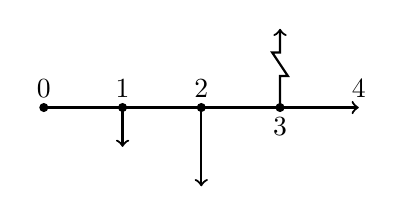
\begin{tikzpicture}
      \draw [->,thick] (0,0) -- (4,0);
      \draw [fill] (0,0) circle [radius=0.05];
      \draw [fill] (1,0) circle [radius=0.05];
      \draw [fill] (2,0) circle [radius=0.05];
      \draw [fill] (3,0) circle [radius=0.05];
      \draw [->, thick] (1,0) -- (1,-0.5);
      \draw [->, thick] (2,0) -- (2,-1);
      \draw [->, thick] (3,0) -- (3,0.4) -- (3.1,0.4) -- (2.9,0.7) -- (3,0.7) -- (3,1);
      \node [above] at (0,0) {0};
      \node [above] at (1,0) {1};
      \node [above] at (2,0) {2};
      \node [below] at (3,0) {3};
      \node [above] at (4,0) {4};
    \end{tikzpicture} \phantom{mm}
  \end{center}
  \caption{A cash flow diagram. The broken line at $t=3$ indicates the net sum of the cash flow at that period.}
\end{marginfigure}
%
A cash flow diagram is a visualization of cash flows and interest over time. Note that $N$ years from time $t$ is the end of period $N$ and beginning of $N+1$.

\section{Cash Flow Analysis}
A \emph{cash flow event} (CFE) is defined as a disbursement (paid) or receipt (received). The discrete cash flow patterns for compound interest factors (CIFs) are:
\begin{enumerate}
  \item \emph{Single}: A single CFE;
  \item \emph{Annuity}: A set of CFEs over a sequence of periods;
  \item \emph{Arithmetic Series}: A set of CFEs that change by a constant amount from one period to the next;
  \item \emph{Geometric Series}: A set of CFEs that change by a constant proportion from one period to the next;
\end{enumerate}
The principle of discrete compounding assumes each CFE occurs at the end of a period such that a payment at $t$ occurs at the end of period $t-1$.
%
\begin{marginfigure}
  \begin{center}
    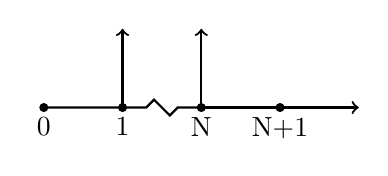
\begin{tikzpicture}
      \draw [thick] (0,0) -- (1.3,0) -- (1.4,0.1) -- (1.6,-0.1) -- (1.7,0) -- (2,0);
      \draw [->, thick] (2,0) -- (4,0);
      \draw [fill] (0,0) circle [radius=0.05];
      \draw [fill] (1,0) circle [radius=0.05];
      \draw [fill] (2,0) circle [radius=0.05];
      \draw [fill] (3,0) circle [radius=0.05];
      \draw [->, thick] (1,0) -- (1,1);
      \draw [->, thick] (2,0) -- (2,1);
      \node [below] at (3,0) {N+1};
      \node [below] at (2,0) {N};
      \node [below] at (1,0) {1};
      \node [below] at (0,0) {0};
    \end{tikzpicture} \phantom{mm}
  \end{center}
  \caption{A cash flow diagram for an annuity over $N$ periods}
\end{marginfigure}
%

\bigskip
The compound amount factor is used for single cash flows, given by \begin{equation}
  (F/P) = (1+i_e)^N = (1+r/m)^{mt}
\end{equation}
The present worth factor is the inverse, $(P/F)$. The sinking fund factor gives the size $A$ of a CFE equivalent to a future amount $F$, given by \begin{equation}
  (A/F) = i / [F/P - 1]
\end{equation}
%
\marginnote{\emph{Annuity Due}: The amount owed from a mortgage is $P = F[(F/P) - (A/P)_{N=12T}(F/A)]$ where $N$ the term and $T$ is the amortization period.}
%
The uniform series compound amount factor is the inverse, $(F/A)$. The \emph{capital recovery factor} gives the value $A$ of such equal periodic CFEs, given by \begin{equation}
  (A/P) = (F/P) (A/F)
\end{equation}
with the inverse being the \emph{series present worth factor}, $(P/A)$. The capital recovery formula accounts for the salvage value $S$, given by \begin{equation}
  A = P(A/P) - S(A/F) = (P-S)(A/P) + Si
\end{equation}
The \emph{annuity due} is the amount lent requiring $N$ monthly payments of $A$ starting today at an annual rate of $i$, such that $P = A + A(P/A)_{N-1}$. The \emph{arithmetic gradient to annuity factor} is given by \begin{equation}
  (A/G) = i^{-1} - N/[F/P - 1] \iff A_{tot} = A' + G(A/G)
\end{equation}

\section{Geometric Series}
The present worth of a geometric series is \begin{equation}
  P = \sum \frac{A(1+g)^{j-1}}{F/P}
\end{equation}
Let the growth-adjust rate $i^\circ = (1+i)/(1+g)-1$. The geometric gradient series to present worth factor is thus \begin{equation}
  (P/A)_g = (P/A)_{i^\circ} / (1+g)
\end{equation}
There are four possible scenarios for gradients series:
\begin{enumerate}
  \item $i>g>0$ or $g>i>0$; the basic scenarios.
  \item $g=i>0$; then $i^\circ = 0$ and $P = NA/(1+g)$
  \item $g<0$; series id decreasing and $i^\circ > 0$.
\end{enumerate}

\end{document}
